%%%%%%%%%%%%%%%%%%%%%%%%%%%%%%%%%%%%%%%%%%%%%%%%%%%%%%%%%%%%%%%%%%%%%%%%%%%%%%%%
%2345678901234567890123456789012345678901234567890123456789012345678901234567890
%        1         2         3         4         5         6         7         8

\documentclass[letterpaper, 10 pt, conference]{ieeeconf}  % Comment this line out if you need a4paper


%\documentclass[a4paper, 10pt, conference]{ieeeconf}      % Use this line for a4 paper

\IEEEoverridecommandlockouts                              % This command is only needed if 
                                                          % you want to use the \thanks command

\overrideIEEEmargins                                      % Needed to meet printer requirements.

%In case you encounter the following error:
%Error 1010 The PDF file may be corrupt (unable to open PDF file) OR
%Error 1000 An error occurred while parsing a contents stream. Unable to analyze the PDF file.
%This is a known problem with pdfLaTeX conversion filter. The file cannot be opened with acrobat reader
%Please use one of the alternatives below to circumvent this error by uncommenting one or the other
%\pdfobjcompresslevel=0
%\pdfminorversion=4

% See the \addtolength command later in the file to balance the column lengths
% on the last page of the document

% The following packages can be found on http:\\www.ctan.org
%\usepackage{graphics} % for pdf, bitmapped graphics files
%\usepackage{epsfig} % for postscript graphics files
\usepackage{mathptmx} % assumes new font selection scheme installed
%\usepackage{times} % assumes new font selection scheme installed
\usepackage{amsmath} % assumes amsmath package installed
\usepackage{amssymb}  % assumes amsmath package installed
\usepackage{multicol}
\usepackage[bookmarks=true]{hyperref}
\usepackage{mathptmx}
\usepackage[T1]{fontenc}
\usepackage{authblk}
\usepackage{graphicx}
\usepackage{relsize}		% For \smaller
\usepackage[linesnumbered]{algorithm2e}
\usepackage{subcaption}
\usepackage{makecell}
\usepackage{pgfplots}
\usepackage{multirow}
\usepackage{booktabs,caption}
\usepackage[flushleft]{threeparttable}
\usepackage{epsfig}

%commands
\DeclareRobustCommand{\rchi}{{\mathpalette\irchi\relax}}
\newcommand{\irchi}[2]{\raisebox{\depth}{$#1\chi$}} %

\newcommand{\marc}[1]{\textbf{\texttt{\color[rgb]{0,0,.8}#1}}}

\DeclareMathOperator*{\maxB}{max} % Jan Hlavacek
\DeclareMathOperator*{\argmaxB}{argmax}   % Jan Hlavacek
\DeclareMathOperator*{\minB}{min} % Jan Hlavacek
\DeclareMathOperator*{\argminB}{argmin}   % Jan Hlavacek

\usetikzlibrary{positioning,fit,calc}
\tikzset{
block/.style={
draw,
thick,
text width=1.1cm,minimum height=1.5cm,align=center},
line/.style={-latex},
font={\fontsize{8pt}{12}\selectfont}
}

%title
\title{\LARGE \bf
Combined Task and Motion Planning under Partial Observability: An Optimization based Approach
}


\author{\textbf{Camille Phiquepal \space\space\space\space\space\space\space\space\space\space\space\space Marc Toussaint}\\
Machine Learning \& Robotic Lab, University of Stuttgart\\
\{firstname.surname\}@ipvs.uni-stuttgart.de
       }


\begin{document}



\maketitle
\thispagestyle{empty}
\pagestyle{empty}


%%%%%%%%%%%%%%%%%%%%%%%%%%%%%%%%%%%%%%%%%%%%%%%%%%%%%%%%%%%%%%%%%%%%%%%%%%%%%%%%
\begin{abstract}

%We present new algorithms \marc{multiple?} for Task and Motion Planning (TAMP) under partial observability. Our approach builds upon the Logic-Geometric Programming approach (LGP) presentend in prior work, and extends the framework to handle partial observability. We model the problem as a particular kind of POMDP (Partially Observable Markov Decision Process) that we solve assuming a start belief state. Trajectory cost and constraint functions are associated to each action. These functions link symbolic actions with continuous geometric motions. The reward of an action is defined as the negative costs of the optimal trajectory defined by these functions. \marc{I'm still not sure about calling this reward: the path cost is not a sum of independent step rewards; but in a Markovian MDP, all rewards are independent per step. If at all, path costs relate to return. No?} Reward evaluation requires motion planning and is costly to compute. The presented algoritm aims at optimizing policies while limiting the number of reward computations (motion planning queries). Our method explores the policy space in an iterative process. Motion planning is used to evaluate policies. Task planning decides which policy should be evaluated next. The trajectories of the best policy are re-optimized jointly as a holistic optimization problem. To enable the robot to explore its environment, we add ``perceptual actions'' (for example Look) to the robot's classic actions (Pick, Place, etc.) used for manipulation problems. The perceptual actions aim at placing the robot sensor where it can gain information. We evaluate our approach in simulation on object manipulation and autonomous driving examples.
%\marc{shorten the abstract}
We present a new algorithm for Combined Task and Motion Planning (TAMP)
 under partial Observability. Our approach builds on the Logic-Geometric-Programming framework (LGP) presented in prior work [1, 2]. To represent partial observability,
we enable the planner to reason about the agent belief-state. The presented algorithm plans long-term policies that react to the observations that the agent receives. The branching factor due to observations implies that policies are not sequential but tree-like. To handle this specificity, we introduce the notion of "trajectory-tree optimization". The algorithm works in two stages :
First, trajectories are optimized piecewise i.e each action is optimized independently. Under this assumption, the decision process is markovian and policies are optimized using Value Iteration and Rmax algorithm.
Secondly, the markovian assumption is relaxed, and the trajectory-tree of the best policy obtained in the first step is re-optimized globally.
We test our approach on autonomous driving and object manipulation examples. To our knowledge, this is the first TAMP approach that computes long-term policies under partial observability and, hence, computes trajectories that are not sequential but arborescent.
\end{abstract}


%%%%%%%%%%%%%%%%%%%%%%%%%%%%%%%%%%%%%%%%%%%%%%%%%%%%%%%%%%%%%%%%%%%%%%%%%%%%%%%%
\section{INTRODUCTION}
%\marc{please do a spellcheck}
Robots must combine the ability to reason symbolically about discrete actions (Task planning) and geometrically about their realization in the real world (Motion planning). Integrated approaches are referred to in the literature as  Task and Motion Planning (TAMP). 
With the exception of  [4] \marc{use bibtex!!! Oh oh}, current TAMP research assumes full observability. However partial observability is pervasive in many real world situations, e.g.\ when objects are hidden or partially hidden. If some objects to manipulate
are inside containers, the robot has to explore its environment to perform its task. Self driving cars face the same problem when operating in the presence of other vehicles limiting the field of view of the ego vehicle.

In this paper we extend the Logic-Geometric Programming approach (LGP) presented in prior work to handle Partial Observability. Under partial observability, policies have branching points due to observations. On the geometric level, it means that Motion Planning consists in optimizing a trajectory-tree i.e.\ trajectories with ramifications. The TAMP algorithm works in two stages : First piecewise optimization and then joint optimization.  During the first stage, the trajectories of actions are optimized independently (piecewise). This allows the problem to be considered as a Partially Observable Markov Decision Process (POMDP) that we solve from a start belief state. We focus on the case where the true start state is uncertain and partially observable, while the transition model of the underlying MDP is not stochastic. The POMDP is solved in an iterative process. It starts with initial heuristic reward values. A policy is computed using Value Iteration. This candidate policy is given to the motion planner. The resulting trajectory costs are used to replace the initial heuristic reward values of the POMDP. This process is iterated until an equilibrium is reached (no more policy improvement). The second stage of the algorithm is the Joint Optimization. The trajectory tree of the best policy obtained in the first stage is re-optimized globally: instead of optimizing the sequential motion of each action in isolation, the whole trajectory-tree is optimized all at once.

%\marc{"updating rewards" doesn't make sense: you either get rewards or not}

\section{RELATED WORK}

Concerning Combined Task and Motion Planning, a number of approaches [5][8][9] rely on
the discretization of the configuration spaces or action/skeleton parameters to leverage CSP methods. Our prior work presented in [1][2] states TAMP problems as an optimization problem. These approaches assume full observability, and plans are linear sequences of actions. To our knowledge, the system developed by Lozano-Perez and Kaebling [4] is the only other TAMP planner considering partial observability. A \textit{Look} action is used to actively move the robot sensor to acquire information. This approach (Hierarchical Planning in the Now) interweaves planning with execution (in the now). Sequences of actions are planned by approximating the system dynamics (results of actions and observations). Replanning is triggered once the robot ends up in a state not covered by the plan. Our approach aims at planning a full policy from the starting state to the final state. In addition, we aim for smooth and locally optimal trajectories.

Planning for autonomous driving also entails a layered decision making process with a combination of symbolic decisions and planning in a continuous space. [6][7] provide a surveys about planning for self-driving cars. To our knowledge, there exists no literature on TAMP approaches for decision making in the automotive context. 

\section{Problem statement}

We model the task planning part as a particular kind of POMDP $(S, A, T, R, \Omega, O, \gamma)$, where $S$ is a set of symbolic states, and $A$ is a set of symbolic actions. Trajectory cost and constraint functions are associated to each action. These functions implicitly define the action reward \marc{return...} and geometric effect of actions: Given a geometric start configuration, the cost and constraint functions of an action define an optimal trajectory. The action reward is the negative cost of this optimal trajectory, the geometric configuration reached after this action is the last configuration of this optimal trajectory.
From this definition, it follows that the transition model is deterministic and that a unique geometric configuration is associated to each reachable symbolic state.

More formally, let $\rchi$ be the configuration space of the whole environment, including the robot and all object configurations.

Let $X_k \in \rchi$ be the geometric configuration at time $t_k$. The agent takes an action $a \in A$ which takes effect over the interval $[t_k, t_{k+1}]$. Costs and constraints functions $f_a, g_a, h_a$ are associated to the action $a$. We call $C(X_k)$, the space of all trajectories starting from $X_k$ over the interval $[t_k, t_{k+1}]$.

The cost of a trajectory $x \in C(X_k)$ under the action $a$ for the time interval $[t_k, t_{k+1}]$ is,
\begin{align*}
c(a, x) = \int_{t_k}^{t_{k+1}} & {f_a(x(t), \dot{x}(t), \ddot{x(t)})dt}\\
s.t\ \  & g_a(x(t), \dot{x}(t), \ddot{x(t)}) <= 0\\
& h_a(x(t), \dot{x}(t), \ddot{x(t)}) = 0 ~.
\end{align*}
The optimal trajectory is: $x^\star = \argminB_{x \in C(X_k)} c(a, x)$\\

The successor geometric configuration $X_{k+1}$ is the last geometric configuration of the optimal trajectory,
\begin{align*}
X_{k+1} = x^\star(t_{k+1}) ~.
\end{align*}
The reward of the action $a$ is the negative trajectory cost of the optimal trajectory if the constraints are satisfied, minus infinity otherwise,
\begin{align*}
R(a, X_k) =\left\{\begin{matrix}
- c(a, x^\star), \text{if $g$ and $h$ satisfied}\\ 
-\infty,\ \text{otherwise}
\end{matrix}\right. ~.
\end{align*}
A belief state is a probability distribution over the state space. Since a geometric configuration is associated to each symbolic state, it is also probability distribution over geometric configurations. In particular, the reward of an action taken in a belief state $b_k$ is
\begin{align*}
 R(a, b_k) = \sum_{X \in b_k} b_k(X) R(a, X) ~.
\end{align*}

\subsection{Decision graph}

When planning from an initial belief state and observations are discrete, the set of all possible reachable belief states is a graph. Each node is a belief state. There are two kinds of nodes: 
\begin{itemize}
\item Action nodes: the agent has to choose which action to take. The edges starting from the node are the different possible actions. The reward received after executing the action is associated to each action-edge.
\item Observation nodes: the agent receives an observation, each edge starting from an observation node is a possible observation.
\end{itemize}

\subsubsection{Example for a decision graph}

We consider a car behind a truck, the car wishes to overtake but cannot see the opposite lane because of the truck, see Fig.~\ref{fig:overtaking}. The car can take three actions: look into the opposite lane, overtake the truck, or continue to follow the truck. After looking into the lane (move slowly toward the center of the road), the car receives an observation (lane free or not). Fig.~\ref{fig:overtaking-decision-graph} is the decision graph of this problem.

%\marc{use the figure environments!! Here is one example:}

\begin{figure}\centering
  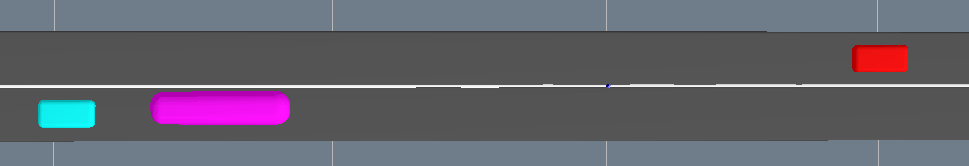
\includegraphics[width=0.5\textwidth]{images/overtaking.png}
  \caption{\label{fig:overtaking} The ego vehicle
    (cyan) wants to overtake but cannot observe if a vehicle arrives
    in the opposite direction because of the truck.}
\end{figure}
    
\begin{figure}\centering
  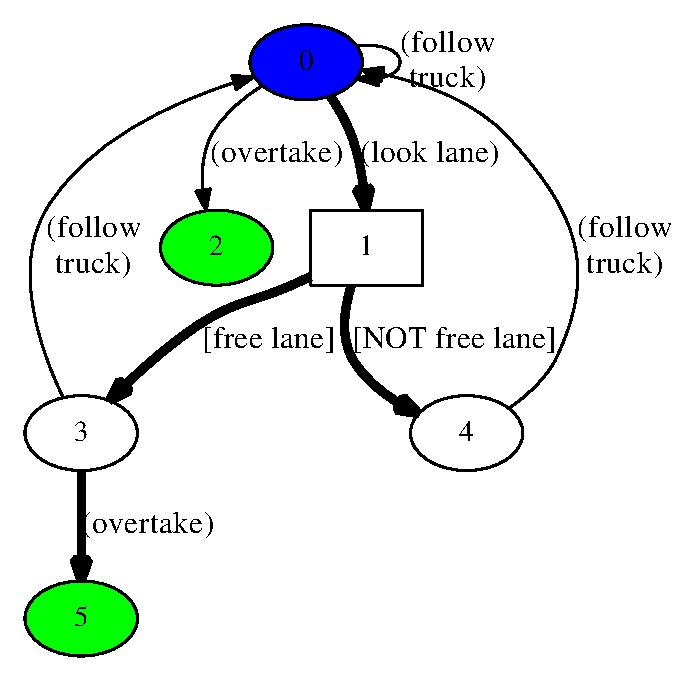
\includegraphics[height=0.25\textwidth]{images/graph.eps}
  \caption{\label{fig:overtaking-decision-graph} Decision graph for overtaking, the thick edges represent a possible policy}
\end{figure}
  
\subsubsection{Policy}

A policy $\pi$ is a mapping from belief states to actions. Optimizing a policy consists in determining the best action at each action node. The thick edges in Fig.~\ref{overtaking-decision-graph} represent a possible policy. The decision graph potentially contains cycles, however, under the assumption, that trajectory costs are always strictly positive, the optimal policy is assured to be a tree (no cycles). In the case of full observability, the policy boils down to a sequence of actions.

%\marc{(not reward)}
The expected return of a policy $\pi$, starting from the belief state $b_0$ and configuration $X_0$, is defined recursively as
%
\begin{equation}
U^{\pi}(b_0) = \\R(a, b_0) + \gamma \sum_{o \in \Omega } O( o | b, a ) U^{\pi}(T(b_0, a, o)) ~.
\end{equation}
%
In the above expression, $\Omega$ refers to the observation space, $O$ refers to the observation model, and $T(b, a, o)$ is the successor belief state after observing $o$. In the example of the last section (\ref{fig:graph}), $b_2 = T(b_0, (look\ lane), [NOT\ lane\ free])$.

The optimal policy is the policy maximizing the return,
\begin{equation}
\pi^{\star} = \argmaxB_{\pi} U^{\pi}(b_0) ~.
\end{equation} 
\marc{please do potential commas before an equation (not :), and . at the end of an equation}

\marc{No, that's not a proper problem statement. What you optimize for here is just the sum of independent piece costs. But what you eventually want is the joint optimum along time, and joint across observations. That's different to summing independent piece costs.}
  
\section{TAMP Algorithm}

Our approach for optimizing a TAMP policy (solve equation (2)) is schematized on Fig.~\ref{fig:algo}. First, the decision graph is built with heuristic reward values. Secondly, iterations of task planning and fast motion planning are performed: Task planning computes a candidate policy based on the last reward values. The policy is given to the motion planner which computes the trajectories and costs of each action. The resulting costs are used to update the rewards associated to the actions. Task planning is re-run which potentially results in a new policy candidate. This process is iterated until an equilibrium is reached (no more policy improvement).

Finally, a pass of joint trajectory optimization is performed on the best policy found. This pass doesn't plan each action trajectory in isolation but optimizes the trajectories as a whole. It is typically slower but gives smoother and more optimal results. Different optimization parameters (more time steps) can be used in this final stage.

\begin{figure}
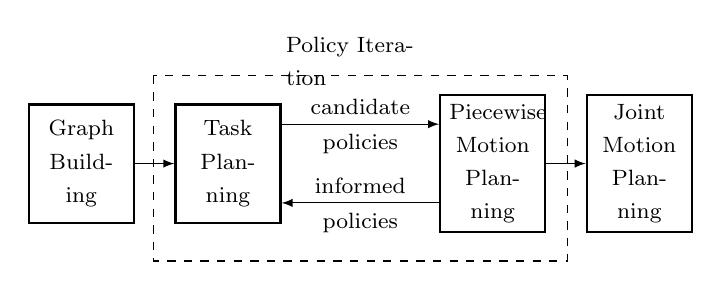
\begin{tikzpicture}
  \node[block] (a) {Graph Building};
  \node[block, right=0.5cm of a] (b) {Task Planning};
  \node[block, right=2cm of b] (c) {Piecewise Motion Planning};
  \node[block, right=0.5cm of c] (d) {Joint Motion Planning};
  %\coordinate [left=of c] (b_output);
  \draw[line] (a)-- (b);
  \draw[line] ([yshift=0.5cm] b.east)-- ([yshift=0.5cm] c.west) node[pos=0.5,above]{candidate} node[pos=0.5,below]{policies};
  \draw[line] ([yshift=-0.5cm] c.west)-- ([yshift=-0.5cm] b.east) node[pos=0.5,above]{informed} node[pos=0.5,below]{policies};
  \draw[line] (c)-- (d);
%  \node (rect) [rectangle, draw, minimum width=70mm, minimum height=100mm, anchor= south west] at (0,0) {};
  \draw [draw=black,dashed] ([xshift=-0.95cm, yshift=0.35cm] b.north) rectangle ([xshift=0.95cm, yshift=-0.35cm,label=$m$] c.south);
%  \draw [decorate,decoration={brace,amplitude=10pt},xshift=0pt,yshift=0pt]
%([xshift=-0.55cm] b.north) -- ([xshift=0.55cm] c.north);
\node[text width=2cm] at (3.6,1.3) {Policy Iteration};
\end{tikzpicture}
\caption{TAMP algorithm}
\label{fig:algo}
\end{figure}

\subsection{Graph Building} 
%\marc{throughout: replace graph by tree?}
The decision graph, is expanded from the start belief state using a breadth first strategy. In the general case, the number of reachable belief states is infinite leading to an infinite decision graph. The algorithm that we present in this paper assumes a graph of finite size. To constraint the graph size to be finite, one solution is to expand the graph up to a certain maximal depth.
%% Under the assumption that both the transition model and the observation model are deterministic, the decision graph is also guaranteed to be finite without restricting the expansion depth. [MARC: that depends on the problem]
%% Under such an assumption, the agent is still faced at with uncertainty due to partial observability.

\subsection{Value Iteration on the decision graph} \label{ssec:dp}
%\marc{use big or bigg in equations, not mathlarger}
Under the optimal policy, the value of each action node obeys the Bellman equation, 
\begin{equation}
V^{\star}(b) = \max_{a} \big[ R(a, b) + \gamma \sum_{o \in \Omega } O( o | b, a ) V^{\star}(T(b, a, o)) \big] ~.
\end{equation} 
At each pass, the algorithm goes through each action node and updates its current value based on the values of its children. The update process is iterated until the values are stable i.e. the Bellman equilibrium has been reached,
\begin{equation}
V^{\star}_{i+1}(b) \leftarrow \max_{a} \big[ R(a, b) + \gamma \sum_{o \in O(b, a) } O( o | b, a ) V^{\star}_{i}(T(b, a, o))
\big] ~.
\end{equation} 
Once the value is know, the optimal policy is retrieved by selecting at each action node the action leading to the children with the highest expected value.

\subsection{Piecewise Motion Planning} \label{ssec:top}

Task Planing gives candidate policies to the motion planner. The execution time of this phase is crucial for the overall planning time. This is performed in two steps, a first feasibility check and, then, trajectory optimization. For these two steps, each action is optimized independently in a breadth-first order. Trajectory Optimization is performed using the Logic Geometric Programming framework (LGP)[1][2]. The results (the trajectory and its cost) are saved, so an action edge is only planned one time. There may be a strong overlap between candidate policies (same edge in many candidate policies). This is especially the case in the last iterations of Policy improvement, but motion planning is performed only on edges that haven't been planned yet. Intuitively, as Policy iteration goes along, the decision graph is filled with geometric information. The initial reward is the parameter which controls how large the coverage will be and how fast convergence occurs. Pose level approximation and re-using results of previous optimizations for the planning of new policies are ways to speed-up the optimization.\\ 

\subsubsection{Pose level optimization} \label{ssec:fast}
To detect quickly infeasible trajectories, we first optimize key-frames only (robot pose at each node). This step is much quicker than optimizing a trajectory. If an action is impossible during the feasibility check, the optimization is not pursued further. This feasibility check is optimistic, it might succeed even if the path itself is infeasible (no possible trajectory without collision between two key-frames for example). Although this gives a feasibility information it doesn't provide with trajectory costs.\\

\subsubsection{Trajectory optimization}
The second pass of optimization consists in optimizing between key-frames, we consider typically 20 time steps for each action. In addition to the cost and constraint functions defined by the action, the robot dynamic and collision avoidance are considered which results in accurate trajectory costs that will update the reward model of the decision graph.

%% \subsection{Backup Mechanism} \label{ssec:backup}

%\marc{I deleted the subsection header 'backup' - I don't understand why you call this backup. Value Iteration is the backup.}

The initial rewards of decision graph are replaced with the trajectory costs resulting from the fast motion planning. The resulting geometric configuration of the robot at the end of each planned action is also saved. The reward of infeasible actions is set to minus infinity which excludes this edge from next candidate policy. 
 
\subsection{Rewards initialization and graph exploration}\label{ssec:explo}
%Rmax Algorithm

\marc{Did you lookup Rmax? You need to compare it to this and describe it in that manner.}
  
The initial rewards influence drastically the search behavior. Optimistic initial rewards encourage exploration. This can be intuitively understood, since unexplored actions have big rewards, the Value iteration tends to converge to a policy having unexplored actions. On the other hand, with pessimistic initial rewards, the equilibrium is attained after a first policy has been successfully optimized by the motion planner. Higher initial rewards converge to better policies at the expense of the overall planning time. 
 
\subsection{Joint Motion Planning}
Optimizing actions independently cannot capture long-term effects on the trajectories. When considering a policy as one single optimization problem, final actions potentially influence motions earlier on the trajectory-tree. The autonomous driving example of the experimental results exemplifies this idea. Moreover, planning parameters (e.g. number of key frames) may be different when planning for informing the search or planning for outputting the final policy. This final stage of optimization allows for reaching a better optimum and smoother motions. Although it takes much longer but this is done on one single policy. \\
Because of the observation branching, the whole motion is a trajectory-tree and is not straightforward to optimize. We solve it in two phases: First, linear trajectories are optimized from the root graph node to each one of the terminal belief states (see $opt\_1$ and $opt\_2$ on Fig.~\ref{fig:joint}). Secondly, the trajectories are re-optimized with additional constraints enforcing that the common parts between trajectories are identical (see $opt\_3$ and $opt\_4$). The re-optimization is potentially performed multiple times until the equality constraints across trajectories are fully satisfied (in practice, one iteration is often enough).
%\marc{weighed $\to$ weighted in the figure}

\begin{figure}[h!]
  \centering
      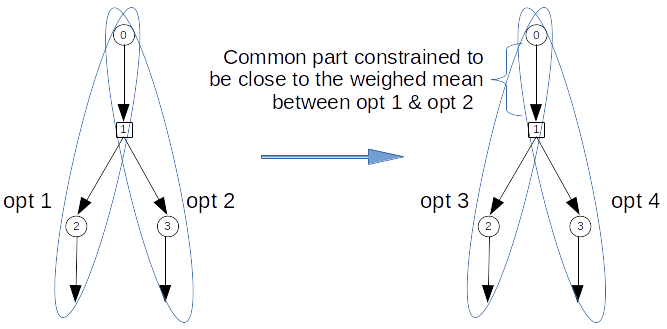
\includegraphics[height=0.2\textwidth]{images/tree-joint_2.png}
  \caption{Joint optimization}
  \label{fig:joint}
\end{figure}

\section{Experimental Results}
\subsection{Overtaking behavior}
We consider the overtaking problem introduced previously. Fig.~\ref{fig:overtaking-decision-graph} is the decision graph and Fig.~\ref{fig:overtaking-start-configurations} shows two start configurations. In the first configuration $(a)$, the opposite lane is free enough to overtake. In $(b)$ overtaking is not possible. The Fig.~\ref{fig:overtaking-policy} shows the optimal policy. The trajectory cost of the action \textit{Look} is implemented as the distance between the car and the center of the road. It tends to move the car toward the center to get sight of the lane (see Fig.~\ref{fig:overtaking-look}). The action \textit{Follow} is implemented as a constraint which is satisfied if the ego-car is behind the truck (with a safety distance) at the end of the action. On the other hand, the action \textit{Overtake truck} is implemented as a constraint satisfied if the ego-car is in front of the truck.
\begin{figure}[h!]
  \centering
      \includegraphics[width=0.5\textwidth]{data/cars/policy.eps}
  \caption{Overtaking optimal policy}
  \label{fig:overtaking-policy}
\end{figure}

\begin{figure}[h!]
  \centering
  \begin{subfigure}[t]{0.5\textwidth}
      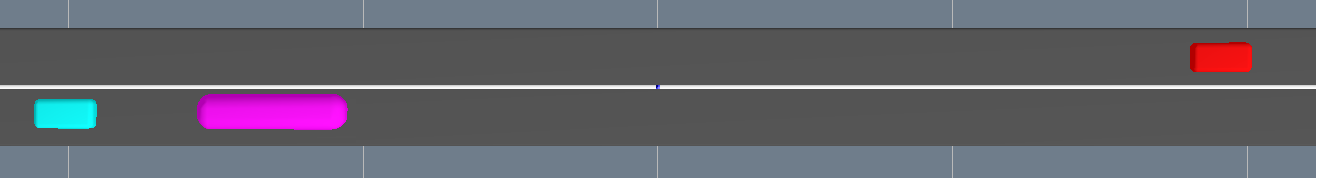
\includegraphics[width=\textwidth]{data/cars/start-0.png}
      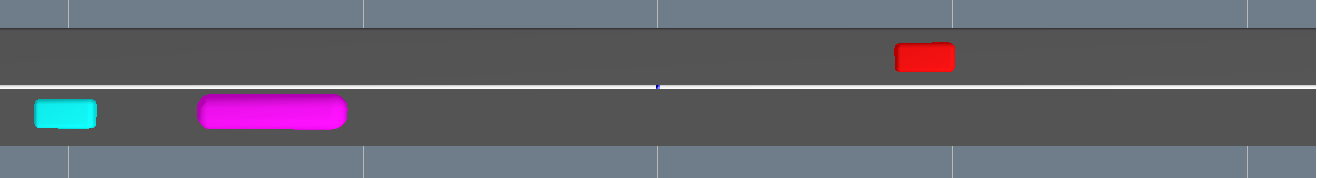
\includegraphics[width=\textwidth]{data/cars/start-1.png}
      \caption{\label{fig:overtaking-start-configurations}two start configurations}
  \end{subfigure}   
      
  \begin{subfigure}[t]{0.5\textwidth}
      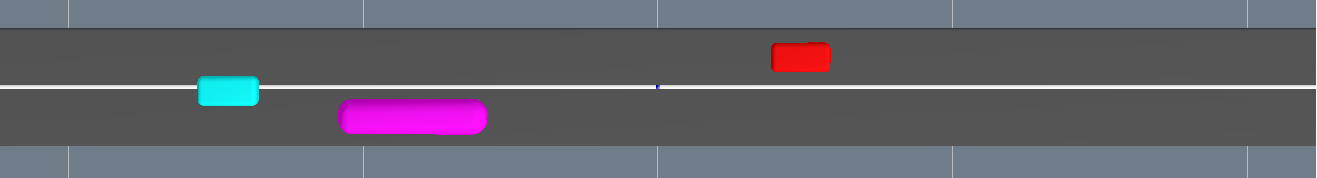
\includegraphics[width=\textwidth]{data/cars/look.png}
        \caption{\label{fig:overtaking-look}\textit{Look} action, the ego vehicle moved to the road center to observe the lanes}   
  \end{subfigure} 
  \begin{subfigure}[t]{0.5\textwidth}
      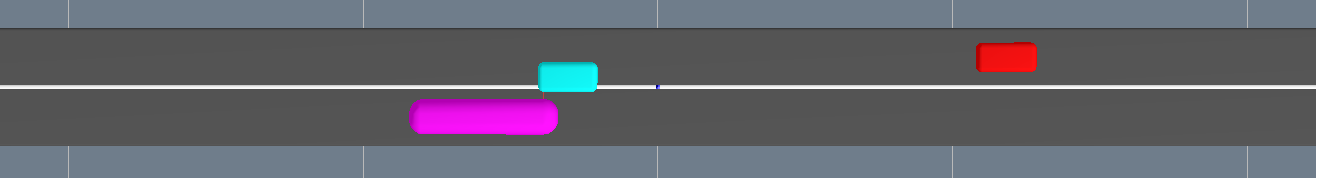
\includegraphics[width=\textwidth]{data/cars/overtaking.png}
        \caption{the ego vehicle overtakes (the opposite vehicle is far enough)}
  \end{subfigure}
  \begin{subfigure}[t]{0.5\textwidth}
      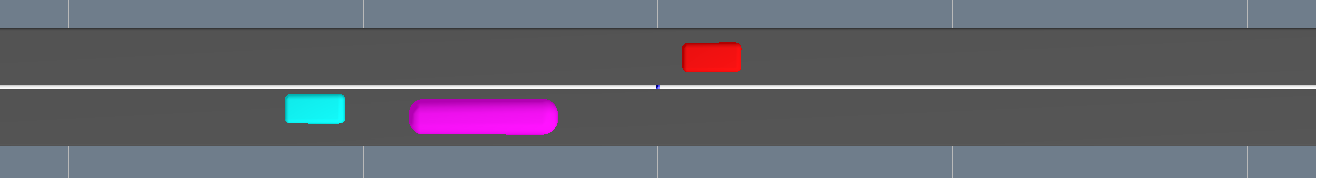
\includegraphics[width=\textwidth]{data/cars/follow.png}
      \caption{the ego vehicle moves back to its lane (opposite lane not free)}
  \end{subfigure}
\end{figure}

This example emphasizes the improvement brought by the joint trajectory optimization. The curves on Fig.~\ref{fig:overtaking-speeds} represent the longitudinal velocities of the trajectory-tree for different planning configurations. At $t=6.5 s$, the car receives the percept $[lane\ free]$ or $[NOT\ lane\ free]$. This is the branching point of the trajectory-tree. If the lane is free, the car accelerates to overtake and then slows down once the truck is overtaken. Otherwise, the car slows down and move back to follow the truck.

\begin{figure}
\begin{tikzpicture}
\begin{axis}[
    %title={Vehicle Speed},
    xlabel={Time(s)},
    ylabel={Speed (m/s)},
    xmin=0, xmax=15,
    ymin=17.5, ymax=47.5,
    xtick={0,5,6.5,10,15},
    ytick={20, 30, 40, 45},
    legend pos=north west,
    legend columns=1,
    legend style={font=\fontsize{7}{8}\selectfont},
    legend cell align={left},
    ymajorgrids=true,
    grid style=dashed,
    x label style={at={(axis description cs:0.5,0.05)},anchor=north}
]
   \addplot[ 
    color=purple,
    style={very thick}
    ]
    table [col sep=comma]{data/cars/30-70/0.csv}node[above,pos=0.56] {$overtaking$};
    \addlegendentry{$ Joint\ Planning\ prior\ of\ p( lane\ free ) = 0.3$}
    
    \addplot[ 
    color=blue,
    style={very thick}
    ]
    table [col sep=comma]{data/cars/70-30/0.csv};
    \addlegendentry{$ Joint\ Planning\ prior\ of\ p( lane\ free ) = 0.7$}
    
    
    \addplot[ 
    color=gray,
    style={very thick}
    ]
    table [col sep=comma]{data/cars/fast/0.csv};
    \addlegendentry{$ Fast\ Motion\ Planning\ only$}
    
    \addplot[ 
    color=purple,
    style={very thick}
    ]
    table [col sep=comma]{data/cars/30-70/1.csv}node[below,pos=0.63] {$following\ truck$};
    %\addlegendentry{$joint 1$}
    
    \addplot[ 
    color=blue,
    style={very thick}
    ]
    table [col sep=comma]{data/cars/70-30/1.csv};
    %\addlegendentry{$ p( lane\ free ) = 0.7$}
    
    \addplot[ 
    color=gray,
    style={very thick}
    ]
    table [col sep=comma]{data/cars/fast/1.csv};
    
\end{axis}
\end{tikzpicture}
  \caption{\label{fig:overtaking-speeds}Longitudinal speed of the overtaking maneuver}
\end{figure}

The gray curve results from the fast motion planning. Actions are optimized in isolation, when looking at the lanes, the car keeps exactly the same speed (gray curve is flat for $t<6.5s$). When starting to overtake, the car is, still quite far from the truck and accelerates strongly to overtake. On the other hand, the blue and purple curves (Joint Optimization) are much smoother. To avoid a too strong acceleration, the car anticipates and accelerates slightly when looking. If overtaking is possible, the car pursues its acceleration, otherwise, it slows down and go back in the lane. We think that this mimics what human drivers do in case of ``tense'' overtaking maneuver. The initial belief state also influences the behavior. If it is likely that overtaking is possible ($0.7$ likelihood for the blue curve), the car will accelerate more when looking. In practice, the initial belief state could come from a service providing global information about the traffic in the area.

\subsection{Sussman anomaly under partial observability}
We consider an humanoid robot (see Fig.~\ref{fig:sussman} ). There are three blocks a table. The robot has to stack the blocks in a given color order on one of the three table locations (red on the top, green in the middle, blue at the bottom). We compute trajectories for all the robot joints (27 degrees of freedom). Only the robot left hand is assumed to be able to grasp. The blocks are black with one side colored (assumed to be the opposite side). The robot knows where the blocks are (referred as $block\_1$, $block\_2$, $block\_3$). However it cannot see the colored side from behind and has explore to identify the blocks and to build the stack in the correct order. 
\begin{figure}
\centering
        \begin{subfigure}[t]{0.15\textwidth}
            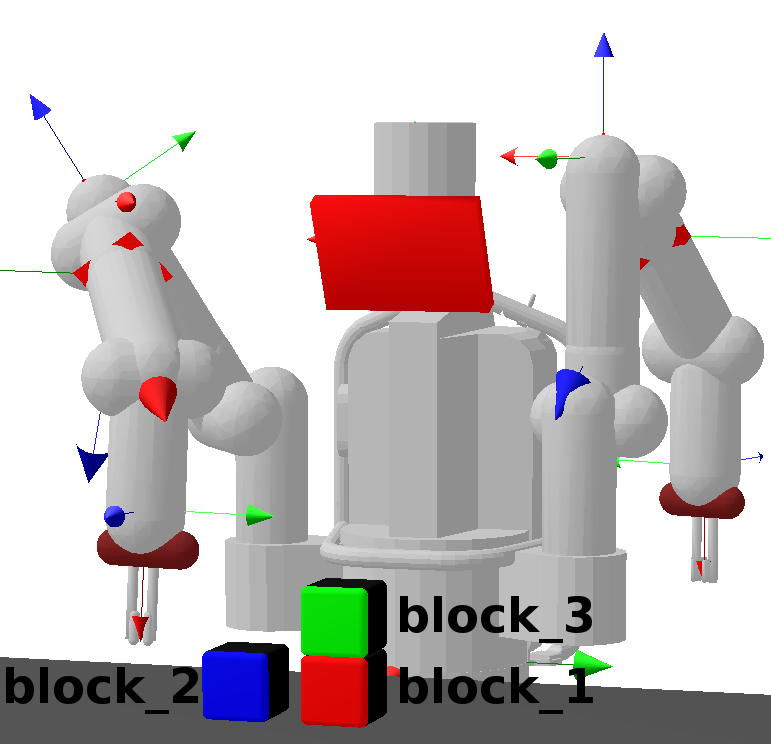
\includegraphics[width=\textwidth]{images/start-a.png}
            \caption{\label{fig:start-1}first start configuration with model B}
        \end{subfigure}
        \hfill
        \begin{subfigure}[t]{0.15\textwidth}
            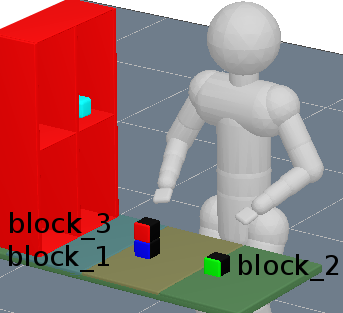
\includegraphics[width=\textwidth]{images/start-b.png}
            \caption{\label{fig:start-2}second start configuration with model B}
        \end{subfigure}
        \hfill
        \begin{subfigure}[t]{0.15\textwidth}
            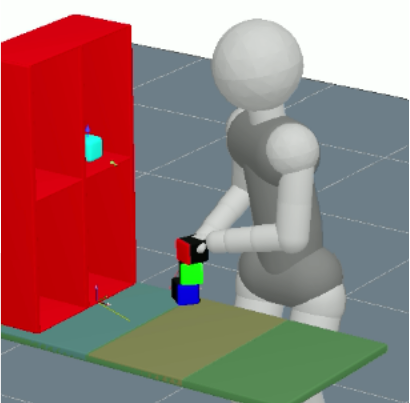
\includegraphics[width=\textwidth]{images/suss-c.png}
            \caption{example of goal configuration}
        \end{subfigure}
        \caption{\label{fig:sussman}Example of configurations. The robot must stack the blocks in a given color order. The block colors are not visible from behind}
\end{figure}
The table is subdivided in 3 different locations (table left, center and right), if a block is already at a location, the location is occupied (no block can be added on the same table part). There are 3 possible actions: 
\begin{itemize}
\item \textbf{Look} a block: the robot seeks to align its sensor (robot head) with the colored side of the box. This will typically lead the robot to both move its head and its hand simultaneously (see Fig.~\ref{fig:look-1}). After this action, the agent receives an observation (color of the block).
\item \textbf{Grasp} a block: only the left hand can grasp
\item \textbf{Place} a block at a location: the block is placed at the given table location, or onto another block.
\end{itemize}

We evaluate two different action models. In the first variation (Variation 1), the action \textit{Look} has a symbolic precondition: the robot should be holding a block before checking it. This precondition is not present in the second variation (Variation 2). The \textit{Look} action is possible more often which increases the branching factor and the size of the decision graph. However, most of the time, when the robot doesn't hold a block, the \textit{Look} action is infeasible geometrically: Indeed the robot has to place place its head far ahead and look backwards which is, in most cases, infeasible given the geometrical constraints of the robot. It is however interesting to note, that this is possible in some cases (if the robot has just previously placed the block close to the table border with some orientation see Fig.~\ref{fig:look-2}). In other words, the grasp-precondition is not absolutely necessary to ensure the feasibility of the \textit{Look} action. This variation is used to analyse how our approach works with a more ``free'' albeit not invalid symbolic problem description causing a lot of motion planning failures.

\begin{figure}
\centering
        \hfill
        \begin{subfigure}[t]{0.15\textwidth}
            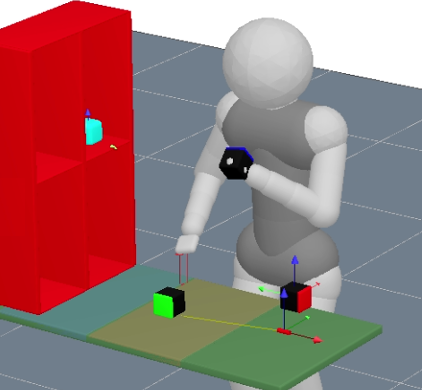
\includegraphics[width=\textwidth]{images/suss-b.png}
            \caption{\label{fig:look-1}\textit{Look} with the block in hand}
        \end{subfigure}
        \hfill
        \begin{subfigure}[t]{0.15\textwidth}
            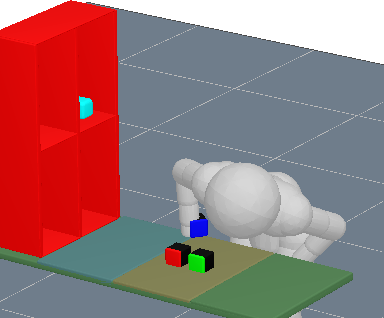
\includegraphics[width=\textwidth]{images/check-no-lift.png}
            \caption{\label{fig:look-2}\textit{Look} just after having posed a block}
        \end{subfigure}
        \hfill
        \caption{\label{fig:checks}Example of geometric configurations reached after the \textit{Look} action}
\end{figure}

To evaluate the scalability, we test with three different initial belief states configurations. In the first configuration (A), the agent has a prior knowledge of the color of each block. This boils down to the fully observable case. To keep the action model unchanged, we still impose that the agent has to look one block to complete its task. In the second configuration (B), 2 blocks are unknown. Fig.~\ref{fig:start-1} and ~\ref{fig:start-2} show the two possible start configurations with this model. In the third case (C), there are no prior knowledge which leads to 6 possible initial configurations. The different start configurations are summed up in the table \ref{table:problems}. In all cases, the initial belief state is uniform (e.g. 1/2 likelihood for each possible start configuration with the model B, 1/6 likelihood for model C).

\begin{center}
\footnotesize
\setlength\tabcolsep{3pt} % default value: 6pt
\begin{tabular}[ht]{|c|c|c|c||c|c|c|}
\hline
\thead{} & \thead{Belief state\\ size} & \thead{Blocks\\known} & \thead{Grasp\\ \textit{precondition}} & \thead{Graph\\size} & \thead{Graph\\building time(s)} \\
\hline
A1                    &  \thead{3/3} & 1 &\thead{yes} &  192 & 0.20 \\
\hline
A2                    &  \thead{3/3} & 1 &\thead{no} &  192 & 0.24 \\
\hline
B1                    &  \thead{1/3} & 2 &\thead{yes} &  336 & 0.53 \\
\hline
B2                    & \thead{1/3} & 2 &\thead{no} &  480 & 1.08 \\
\hline
C1                    & \thead{0/3} & 6 &\thead{yes} &  2076 & 8.55 \\
\hline
C2                    & \thead{0/3} & 6 & \thead{no} &  4128 & 34.3 \\
\hline
\end{tabular}
\captionof{table}{\label{table:problems}Summary of the considered problem variations} 
\end{center}

Fig.~\ref{fig:policy-B2} shows an optimized policy for the model B. The agent first grasps a block and looks it. Once the block is identified, the agent pursues the stacking.

\begin{figure}[h!]
  \centering
  \hfill
  \begin{subfigure}[t]{0.31\textwidth}
      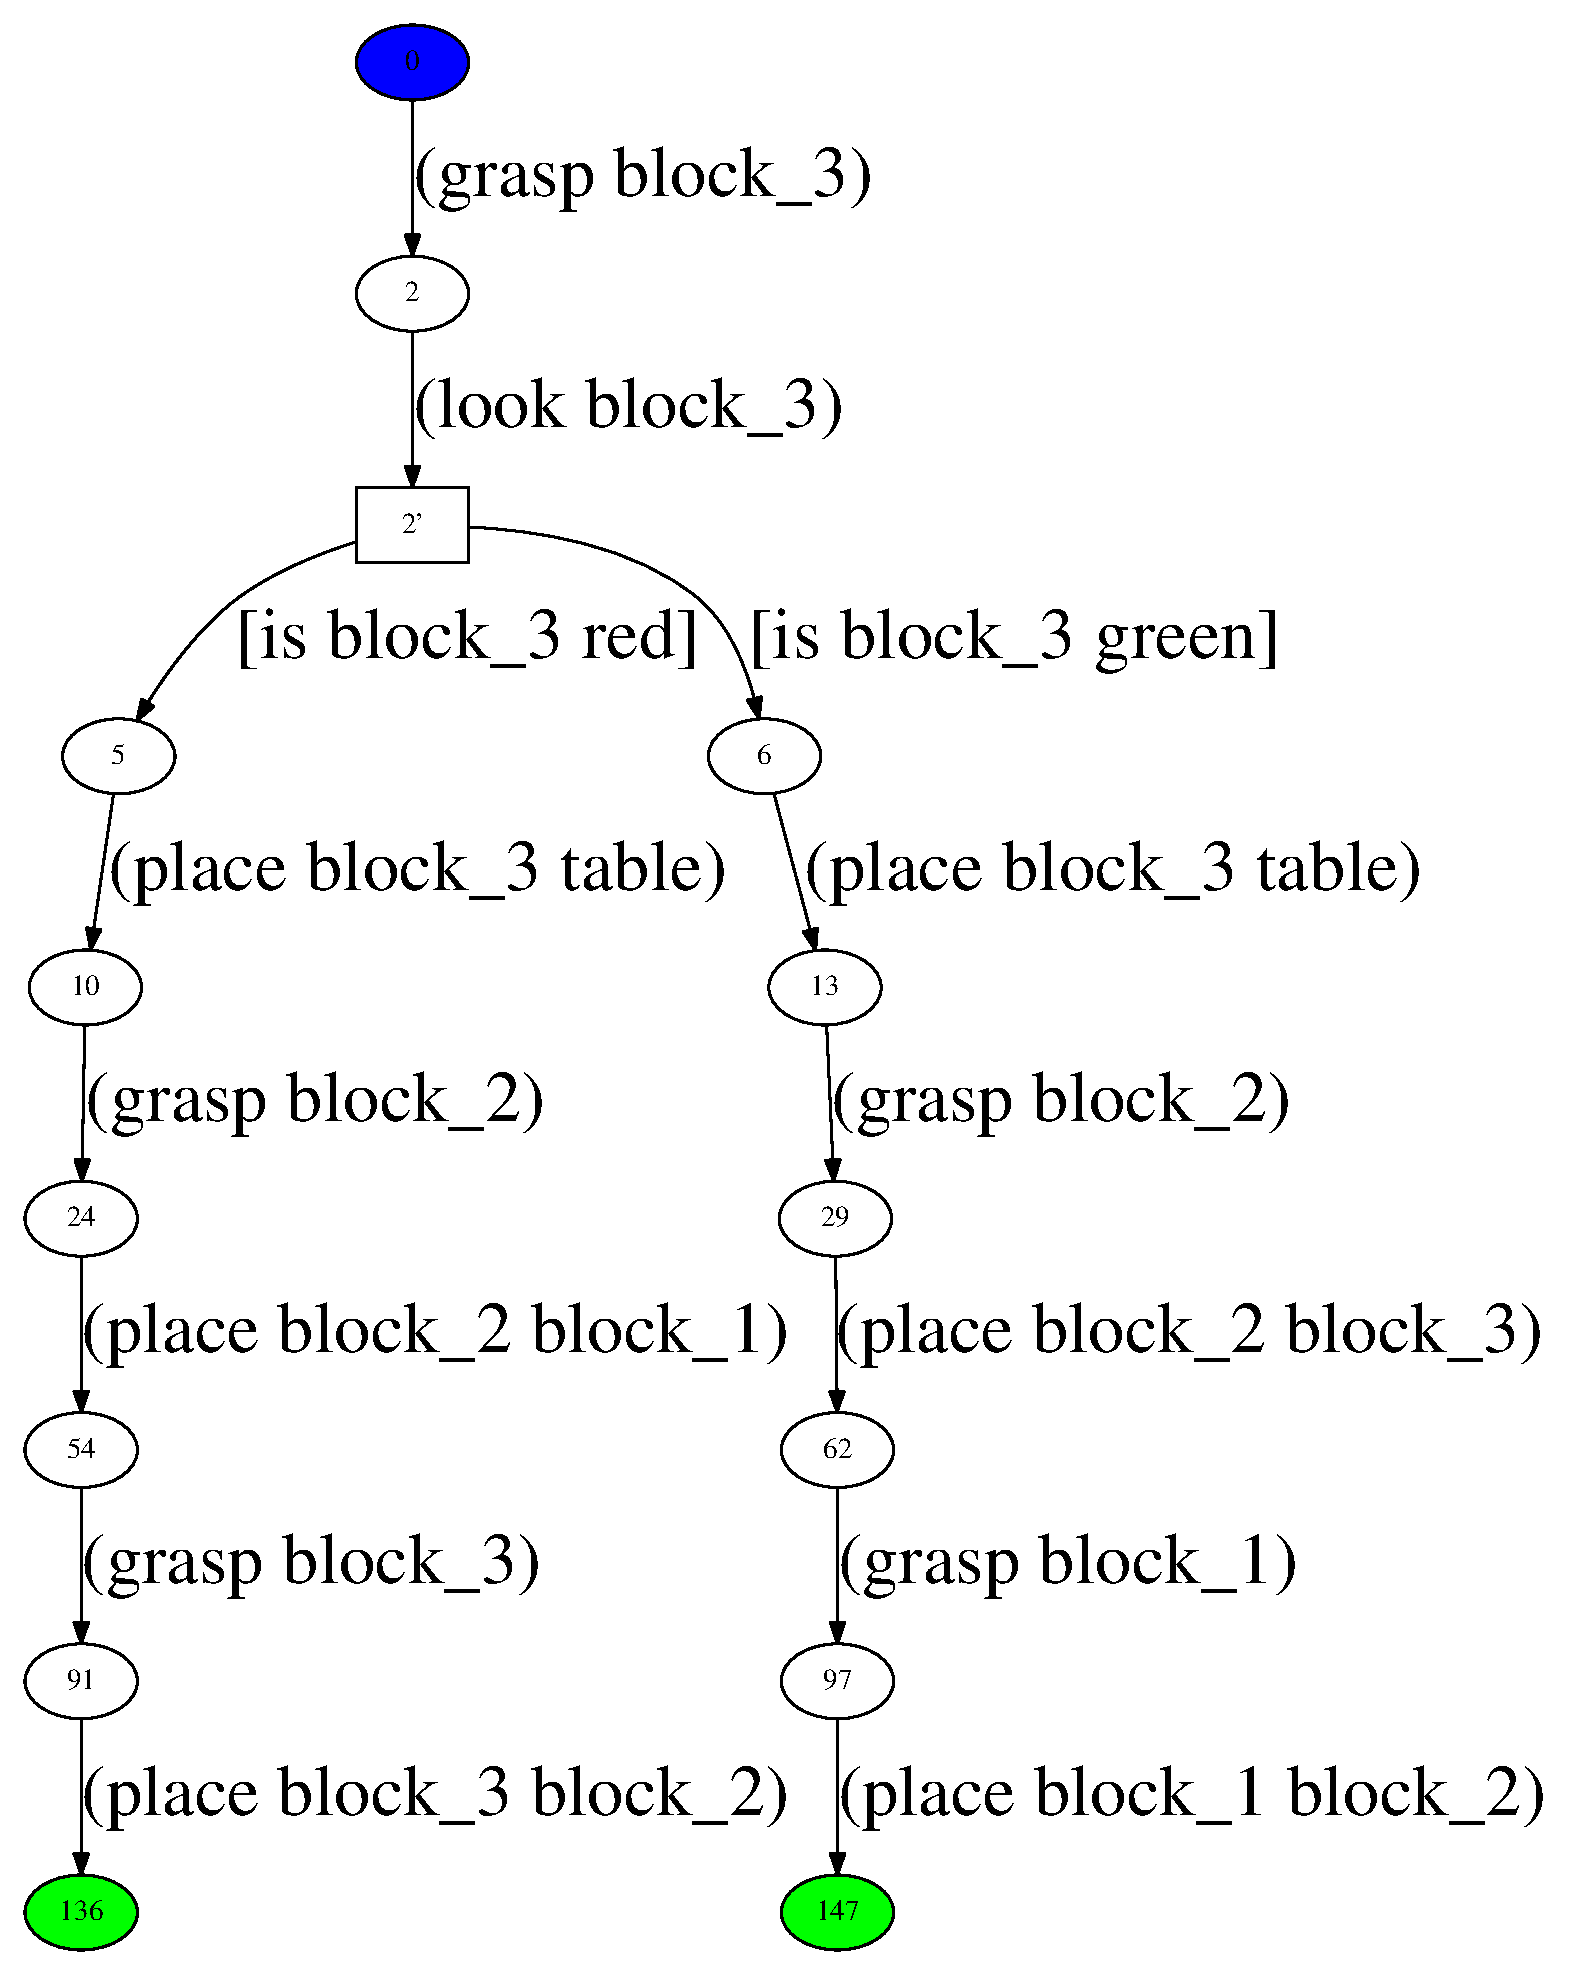
\includegraphics[width=\textwidth]{data/2m1/-0.015/10/policy-11-final-arranged.eps}
  \caption{\label{fig:policy-B2}result policy for B2}
  \end{subfigure}
  \hfill
  \begin{subfigure}[t]{0.15\textwidth}
      \includegraphics[width=\textwidth]{data/1m2/-0.25/10/policy-2-final.eps}
  \caption{\label{fig:policy-A2}result policy for A2}
  \end{subfigure}
\end{figure}

\begin{center}
\footnotesize
\setlength\tabcolsep{3pt} % default value: 6pt
\begin{tabular}{|c|c|c|c|c|c|c|c|}
\hline
                  			   & \thead{$R_0$} & \thead{Iter-\\ations} & \thead{N of\\actions*} & \thead{Task\\planning} & \thead{Fast\\motion\\planning} & \thead{Joint\\motion\\planning} & Total*\\
\hline
\multirow{3}{*}{A1}     & -0.25  & 1 & 7 & 0.007 & 1.37 & 11.4 & 13.0 \\
				        & -0.1   & 2 & 7 & 0.018 & 3.14 & 9.7  & 13.1 \\
					    & -0.015 & 13 & 7 & 0.10  & 18.5 & 16.3 & 35.1 \\
\hline
\multirow{3}{*}{A2}     & -0.25  & 2 & 7 & 0.013 & 1.81 & 8.43 & 10.5 \\
				        & -0.1   & 3 & 7 & 0.019 & 2.08 & 11.6 & 14.0 \\
					    & -0.015 & 16 & 7 & 0.10 & 14.8 & 11.4 & 26.6 \\
\hline
\multirow{3}{*}{B1}     & -0.25  & 1 & 12 & 0.014 & 2.72 & 26.2 & 29.5 \\
				        & -0.1   & 1 & 12 & 0.016 & 2.85 & 21.5 & 24.9 \\
					    & -0.015 & 11 & 12 & 0.13 & 30.6 & 20.6 & 51.9 \\
					    
\hline
\multirow{3}{*}{B2}     & -0.25  & 7 & 12 & 0.089 & 9.10 & 56.7 & 66.9 \\
				        & -0.1   & 14 & 12 & 0.17 & 20.4 & 59.9 & 81.4 \\
					    & -0.015 & 39 & 12 & 0.55 & 69.9 & 38.6 & 110.1 \\
\hline
\multirow{3}{*}{C1}     & -0.25  & 1 & 33 & 0.077 & 11.6 & 172.3 & 192.5 \\
				        & -0.1   & 8 & 33 & 0.35 & 56.9 & 105.5 & 170.9 \\
					    & -0.015 & 41 & 37 & 2.07 & 321.3 & 112.7 & 444.1\\
\hline
\multirow{3}{*}{C2}     & -0.25  & 15 & 33 & 1.16 & 42.4 & 100.8 & 182.8 \\
				        & -0.1   & 48 & 33 & 3.38 & 146.5 & 250.9 & 436.6 \\
					    & -0.015 & 303 & 39 & 26.0 & 1188.9 & 261.5 & 1510.9 \\
\hline
\end{tabular}
\begin{tablenotes}
      \footnotesize
      \item * Number of actions of the final policy
      \item ** The total planning time also includes the graph building time given in the table \ref{table:problems}
    \end{tablenotes}
\captionof{table}{\label{table:times}Number of iterations and planning times} 

\end{center}

\begin{figure}[h!]
\begin{tikzpicture}
\begin{axis}[
    title={Values of candidate and result policies for B1},
    title style={yshift=-2ex},
    xlabel={Iterations},
    ylabel={Value},
    xmin=0, xmax=14,
    ymin=-2, ymax=0.6,
    xtick={0,1,5,10,15,20},
    ytick={-2,-1.5,-1,-0.5,0,0.5},
    legend pos=north west,
    legend columns=2, 
    legend style={font=\fontsize{7}{8}\selectfont},
    legend cell align={left},
    ymajorgrids=true,
    grid style=dashed,
    x label style={at={(axis description cs:0.5,0.05)},anchor=north}
]
   \addplot[ 
    color=purple,
    dashed,
    ]
    table [col sep=comma]{data/2m1/-0.25/10/policy-candidates.data};
    \addlegendentry{$candidate, R_0=-0.25$}
    
\addplot[ 
    color=purple,
    ]
    table [col sep=comma]{data/2m1/-0.25/10/policy-results.data};
    \addlegendentry{$results, R_0=-0.25$}
    
\addplot[ 
    color=blue,
    dashed,
    ]
    table [col sep=comma]{data/2m1/-0.1/10/policy-candidates.data};
    \addlegendentry{$candidate, R_0=-0.1$}
    
\addplot[ 
    color=blue,
    ]
    table [col sep=comma]{data/2m1/-0.1/10/policy-results.data};
    \addlegendentry{$results, R_0=-0.1$}    
 
\addplot[ 
    color=orange,
    dashed,
    ]
    table [col sep=comma]{data/2m1/-0.015/10/policy-candidates.data};
    \addlegendentry{$candidate, R_0=-0.015$}
    
\addplot[ 
    color=orange,
    ]
    table [col sep=comma]{data/2m1/-0.015/10/policy-results.data};
    \addlegendentry{$result, R_0=-0.015$}
             
\end{axis}
\end{tikzpicture}

\begin{tikzpicture}
\begin{axis}[
    title={Values of candidate and result policies for B2},
    title style={yshift=-2ex},
    xlabel={Iterations},
    ylabel={Value},
    xmin=0, xmax=40,
    ymin=-2, ymax=0.6,
    xtick={0,5,10,15,20,25,30,35,40},
    ytick={-2,-1.5,-1,-0.5,0,0.5},
    legend pos=north west,
    legend columns=2,
    legend style={font=\fontsize{7}{8}\selectfont},
    legend cell align={left},
    ymajorgrids=true,
    grid style=dashed,
    x label style={at={(axis description cs:0.5,0.05)},anchor=north}
]
   \addplot[ 
    color=purple,
    dashed,
    ]
    table [col sep=comma]{data/2m2/-0.25/10/policy-candidates.data};
    \addlegendentry{$candidate, R_0=-0.25$}
    
\addplot[ 
    color=purple,
    ]
    table [col sep=comma]{data/2m2/-0.25/10/policy-results.data};
    \addlegendentry{$result, R_0=-0.25$}
           
\addplot[ 
    color=blue,
    dashed,
    ]
    table [col sep=comma]{data/2m2/-0.1/10/policy-candidates.data};
    \addlegendentry{$candidate, R_0=-0.1$}
    
\addplot[ 
    color=blue,
    ]
    table [col sep=comma]{data/2m2/-0.1/10/policy-results.data};
    \addlegendentry{$result, R_0=-0.1$}
     
\addplot[ 
    color=orange,
    dashed,
    ]
    table [col sep=comma]{data/2m2/-0.015/10/policy-candidates.data};
    \addlegendentry{$candidate, R_0=-0.015$}
    
\addplot[ 
    color=orange,
    ]
    table [col sep=comma]{data/2m2/-0.015/10/policy-results.data};
    \addlegendentry{$result, R_0=-0.015$}

\end{axis}
\end{tikzpicture}

\caption{\label{fig:convergences} Policy improvement over iterations}

\end{figure}


\subsubsection{Influence of initial rewards} With an initial reward of -0.25 (pessimistic initial reward), the search finishes as soon as a first policy is found. This happens after one single iteration with the B1. With the B2, the search encounters infeasible actions, the first possible policy is found at the 7th iteration. This policy is less optimal than the results found with the other initial rewards.\\The highest initial reward (-0.015) is always optimistic and leads to the most exploratory behavior. The value of candidate policies (containing at least one unexplored action) are consequently always higher than the result policies (see the orange curves on Fig.~\ref{fig:convergences}. It requires the biggest number of iterations. In particular, task planning also explores deeper policies (with more steps). In some cases a slightly deeper policy results in a better trajectory cost (see B2 with $R_0$ = -0.015). The search converges to a better policy than with the other initial reward values. The small improvements in the last iterations are due to small rearrangements of the target location when placing blocks (e.g. place a block on table-left instead of table-center). \\

\subsubsection{Influence of the action precondition} Removing the precondition increases strongly the decision graph size, more iterations are needed, and a majority of candidate policies are infeasible geometrically. This is visible on Fig.~\ref{fig:convergences} for the model B2 (below), the curves of result policies are very discontinuous because the majority of them are infeasible. Most of the time, Motion planning fails due to one single action. The policy value is minus infinity, but the resulting rewards of each possible actions still inform the decision graph leading to an overall improvement. The search reaches an optimal policy which is as good as the policy obtained with the model with precondition. We think that this is an important quality of the proposed solution. Adding domain specific knowledge in the task planning (to ensure that motion planning will succeed) speeds up the search. However, in the general case, we think that it is not always possible / convenient to incorporate such geometric reasoning (reachability of a view point, reachability of an object) in the logical reasoning. 

\subsubsection{Execution time and scalability}
The overall planning time is dominated by the motion planning (see table.~\ref{table:times} As long as the model is simple (A or B) or the exploration kept low ($R_0$ = -0.25), motion planning is dominated by the single pass of joint optimization. The execution time of this pass mainly depends on the total number of action steps in the policy and on the belief state size but is independent from the number of iterations occurring before. In the configurations requiring the biggest number of iterations (C1 and C2 with $R_0$ = -0.015), motion planning and the overall planning time are dominated by the fast motion planning phases of the policy improvement iterations. It also appears clearly that scalability is a crucial problematic here. All the parameters of the problem increase drastically with the size of the belief state (graph size, required number of iterations, size of the resulting policy, computation time). Parameterizing the search with a very exploratory behavior may be feasible for problems of small sizes but suffers from the curse of dimensionality. One way to still enable some exploration while maintaining a bounded planning time is to save the best candidate policy planned so far and interrupt the iterations when a given time limit is reached.

\section{Conclusion \& Future Work}
We proposed a new, optimization-based approach to TAMP problems. It handles partial observability by reasoning over the agent + environment belief state and by optimizing trajectory-trees that can account for the observation branching. It can plan policies that combine exploratory actions (mostly sensor trajectories) and exploitative actions (e.g grasp, place). The degree of exploration over the vast space of all possible manipulations policies can be controlled by one single parameter (initial heuristic reward). As motion optimization is time consuming, the ability to quickly detect if an an action is infeasible is crucial and we perform it by performing a fast pose-level optimization. Moreover, the policy iteration process naturally copes with motion planning failures that simply inform the decision graph with the real cost (albeit infinitely big) of a given action. Scalability becomes an issue when the number of manipulations and or the size of the belief state increases. An efficient way to speed-up the search is to have a task-level model that is accurately tailored for the problem to solve (example of the grasp precondition), this prevents too many motion planning failures and limits the branching factor. In future work, we intend to explore, how the task-level model can be refined and learned using the results from multiple planning queries.\\
Our current method computes policies that address every possible outcome during the possibility execution. To scale better, we plan to investigate an approach where the policy is planned only for handling the most probable belief state trajectories. As such a policy couldn't handle every outcome at execution time, re-planning would be triggered once the execution layer detects that the system is evolving toward a belief state which is not covered by the current policy.

%biblio
\begin{thebibliography}{99}

\bibitem{c1} M. Toussaint and M. Lopes, Multi-Bound Tree Search for Logic-Geometric Programming in Cooperative Manipulation Domains. Accepted at ICRA 2017.
\bibitem{c2} M. Toussaint, Logic-Geometric Programming: An Optimization-Based Approach to Combined Task and Motion Planning. In Proc. of the Int. Joint Conf. on Artificial Intelligence (IJCAI 2015), 2015.
\bibitem{c3} Brafman, Ronen I. and Tennenholtz, Moshe: {R-MAX} - a general polynomial time algorithm for near-optimal reinforcement learning. Journal of Machine Learning Research, Volume 3, 213-231, 2003
\bibitem{c4} Leslie Pack Kaelbling, Tomas Lozano-Perez. Integrated Task and Motion Planning in Belief Space, International Journal of Robotics Research, 2013
\bibitem{c5} T. Lozano-P�rez and L. P. Kaelbling. A constraint-based method for solving sequential manipulation planning problems. In Intelligent Robots and Systems (IROS 2014), 2014 IEEE/RSJ International Conference on, pages 3684-3691. IEEE, 2014
\bibitem{c6} Katrakazas, C., Quddus, M., Chen, W.-H., Deka, L.: Real-time motion planning methods for autonomous on-road driving: State-of-the-art and future research directions. Transp. Res. Part C 60, 416-442, 2015
\bibitem{c7} Paden, B., Cap, M., Yong, S.Z., Yershov, D., Frazzoli, E.: A survey of motion planning and control techniques for self-driving urban vehicles. IEEE Trans. Intell. Veh. 1(1), 33-55, 2016
\bibitem{c8} F. Lagriffoul, D. Dimitrov, A. Saffiotti, and L. Karlsson. Constraint propagation on interval bounds for dealing with geometric back-tracking. In Intelligent Robots and Systems (IROS), 2012 IEEE/RSJ International Conference on, pages 957-964. IEEE, 2012
\bibitem{c9} F. Lagriffoul, D. Dimitrov, J. Bidot, A. Saffiotti, and L. Karlsson. Efficiently combining task and motion planning using geometric constraints. The International Journal of Robotics Research, 2014






\end{thebibliography}




\end{document}
